\chapter{Introduction}\label{chp:introduction}

The web is becoming the primary platform for all communication, as people gradually move away from solutions provided by their telco operator, such as telephony and text messaging. Moving audio conversations to the Internet has been relatively easy, but as we're now commoditizing video conversations, moving away from custom rooms and dedicated hardware over to regular laptops and phones, the most straightforward solutions lead to performance requirements greater than most user equipment and their connections can handle.

There are lots of competing products on the market today, with different characteristics and performance levels. What they all have in common however, is that they've all chosen a fixed network topology, which dictates most of their expected performance. The goal of this thesis is to investigate the feasibility of designing a system which does not have a fixed topology, but chooses one adaptively based upon properties of the user equipment and connection quality in a given conversation to maximize \emph{utility} of the service to users. To maximize utility, we need to have a well-defined sense of what that implies.


\section{Utility}

\begin{description}

    \item[utility]  The ability of a commodity to satisfy needs or wants; the satisfaction experienced by the consumer of that commodity.\todo{[minor] If time, add phonetic}
\end{description}

When a user evaluates the utility of a video conference service, context is everything. You have different expectations to audiovisual quality on a desktop computer with fiber connectivity compared to your phone on 3G. But how can this difference be quantized? Certainly it's not a question of screen resolution, as most smart phones today have the same 1080p resolution as most computer screens. Resolutions beyond 1080p, like we can find on some ``retina'' screens, are not that interesting for video conferencing, as the webcam producing the source video is unlikely to able to to the full potential of the screen.

However, physical screen size matters. Viewing distance matters. Latency matters very much. Bandwidth matters. Packet loss matters. Most of these should be fairly easy to estimate, but then we have a new problem: which of these attributes do we prioritize? Finding the optimal balance is the key to optimizing service utility. There are of course also non-technical factors that affects the expected experience quite much that cannot be determined by the device itself. For example, even though the device is the same, you'll have different expectations sitting on the bus to work compared to sitting in a sofa in your living room, even though the device and maybe even the connection is the same. Content matters. Environment matters. Mood matters. Time of day probably matters. We will however not take all of these factors into account, but limit our scope to the device and the connection, and since the intended platform is WebRTC, what we can relatively easily determine through a web browser.

We assume that for each user, his experienced utility of the service will be a function of these variables that will follow the general shape of \autoref{fig:utility}. The important point here is the shape of the graph, it's diminishing returns in practice. For smaller devices these will set in earlier, but they have to be present. This ensures that our algorithm will be able to maximize this value over the entire graph, and the results will come back with fairness as to each device's potential.

\begin{figure}
    \centering
    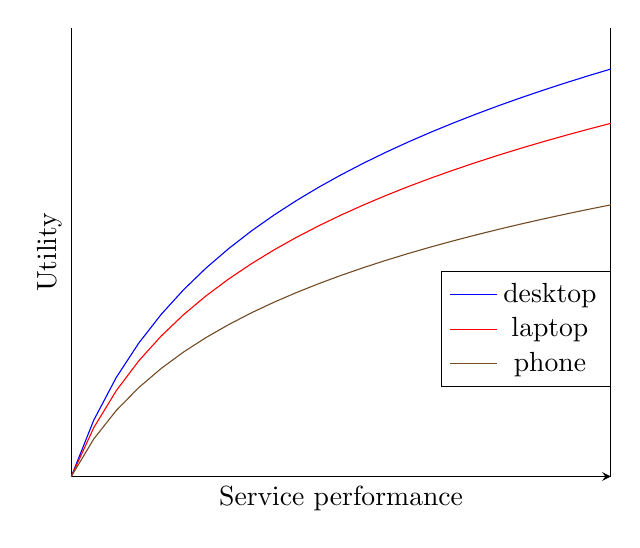
\begin{tikzpicture}
        \begin{axis}[
            xlabel=Service performance,
            ylabel=Utility,
            xmin=1,
            xmax=10,
            ymin=0,
            x axis line style={->},
            ticks=none,
            major x tick style = {opacity=1},
            minor tick length=0pt,
            axis x line=bottom,
            legend style={at={(1,0.20)}, anchor=south east,legend columns=1},
            ]

            \addplot+[domain=1:10,mark=none]{1.5*ln(x)};
            \addlegendentry{desktop}

            \addplot+[domain=1:10,mark=none]{1.3*ln(x)};
            \addlegendentry{laptop}

            \addplot+[domain=1:10,mark=none]{ln(x)};
            \addlegendentry{phone}

        \end{axis}
    \end{tikzpicture}
    \caption{Utility as a function of performance for different devices}
    \label{fig:utility}
\end{figure}


\section{Structure of This Thesis}

To limit the scope of what we're trying to accomplish, we'll define some test cases in \autoref{chp:background} that we'll use throughout the thesis. We'll also evaluate some of the current providers on the market today, and in \autoref{experiments} we'll put one of them to the test, running all the test cases we defined previously to see how the service performs. Knowing this benchmark helps us evaluate the potential for our solution, which we'll take a look at in \autoref{chp:suggested-solution}. We'll discuss how our solution can be implemented, strengths and weaknesses in \autoref{discussion}, before summarizing what we've learned in \autoref{chp:suggested-solution}.


\section{Contribution}

This thesis proposes one way of modelling video conferences with known inter-node latencies and bandwidths as a flow network, and shows how an optimal routing for video can be derived from the model using linear programming. The method also demonstrates how performance can get a significant boost by adding extra nodes to the flow network acting as repeaters and transcoders, bridging the performance gap between traditional \gls{mcu}-backed solutions and peer-to-peer solutions.

We also benchmark the two most popular web browsers as of the time of writing, Google Chrome and Mozilla Firefox in some hard test cases, and reveal severe flaws in how Firefox handles constrained nodes, and lots of potential for increased performance for both browsers. These tests were run with tools developed for this purpose, which are included in the appencies.


\section{Previous and Related Work}

\epigraph{If I have seen further, it is by standing on the shoulders of giants}{Isaac Newton}

Networking and algorithms related to networking is not a new topic, by any stretch of the imagination, and like in all most branches of computer science, it's mostly old problems in a new context.

During this thesis we will borrow heavily from previous work on networking and graph algorithms in general, and flow algorithms in particular. Many algorithmic problems can be solved as a linear program, which as a problem was first solved by Fourier in 1827 \cite{sierksma2001linear}. Another solution, the simplex method, was first introduced by G.B. Dantzig in 1947 \cite{sierksma2001linear}, and was first introduced to me in \cite{ahuja1988network} by Ahuja, Magnanti and Orlin, and serves as the basis for much of our suggested solution. The simplex method has been widely adopted for its ease of implementation on computers, and years of exponential growth of computer performance has made increasingly large problem sets solvable in realistic time.

A study at Chalmers in 2014\cite{tree-topology-webrtc} investigated the feasibility of utilizing normal nodes in a video conference as supernodes, routing traffic from less powerful nodes through these nodes to reduce network load. The authors conclude that such a solution is feasible given proper supernode selection, which gives even greater possibilities for a solution utilizing dynamic topologies like presented in this thesis. Pushing as much traffic as possible over client-provided supernodes lowers the cost for the provider, and enables better quality for the users since peers can be closer to each other than to the closest data center. As the study concluded with supernodes being feasible and beneficial, our method is developed to be flexible enough to allow nodes to forward video to other nodes.

Now that we've established the problem domain and have some grasp of the main challenges, let's see where we are today.


\section{Disclaimer}

This thesis does not try to measure or optimize for audio transmission, as that's a much simpler problem that can practically always be completed by sending the same stream to all nodes in the conversation. There's always only one stream to encode, it doesn't noticably affect available bandwidth, and it's already widely deployed. However, results we achieve for video can also be applied to audio streams if the environment is very heavily constrained or further optimization is required, it's just not the focus of this thesis.
